\chapter{\label{chp:background}Theory and background}
Some theory and background are needed to get a thorough understanding of the material to follow in the following chapters. Some parts of this background chapter were written as part of the specialization project \cite{holm2015pro}, but it is included here to allow the report to be a freestanding document. Some sections has been extended to add a deeper level of understanding to some of the described concepts, compared to what was presented in the previous report. Some information from section 3.3 of the \textit{Methodology}-chapter has also been included in \cref{sec:toolflowbg} of this report, as it describes part of the same tool-flow used here.

In the early days of digital hardware design, gate design and layout were performed by hand. With the rapid growth in the numbers of transistors per digital chip-design, this method quickly became too time-consuming and the need for new and more automated design methods rose. \gls{rtl}-design using \gls{hdl} has long been the standard in digital hardware design. With the increasing demand for low power and small area in large \gls{soc} designs with multiple billion transistors, this methodology is no longer sufficient if hardware manufacturers want to hit the window of opportunity with their state-of-the-art product.

\section{\label{sec:hls}High-Level Synthesis}

\gls{hls} is not a new concept as it were introduced in research papers in the late 1970s and further researched and developed in the 1980s and early 1990s \cite{martin2009high}. The available commercial \gls{hls} tools have not been providing the necessary performance and benefits over \gls{hdl} development for major hardware development companies to adapt this methodology until recently.
The concept of \gls{hls} starts with a functional specification of the circuit described using a higher abstraction level, often a \gls{hll}. A tool use target architectural model libraries and design constraints to transform this specification into hardware, represented as a \gls{rtl} or \gls{hdl}-model. The typical \gls{hls}-flow is shown in figure \ref{fig:hlsflow} and each of the transition-steps is described in the below subsections. The input libraries contain information on available hardware resources with power, area, and delay models for the target architecture.

\begin{figure}[hbpt]
\centering
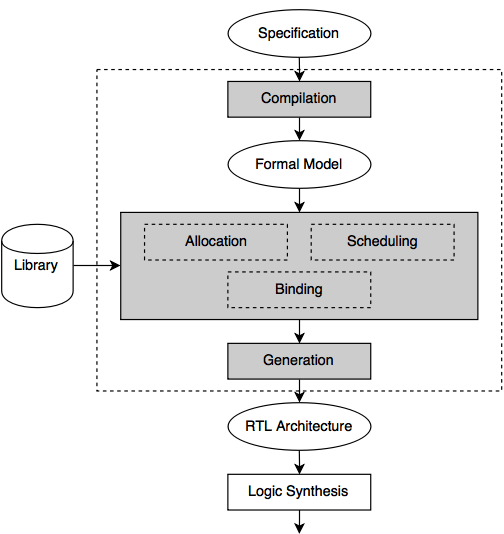
\includegraphics[width=0.55\textwidth]{../figs/HLSFlow.png}
\caption{\label{fig:hlsflow}Information flow in a typical HLS-tool \cite{coussy2009introduction}.}
\end{figure}

\subsubsection{Compilation}

The first step of \gls{hls} is to compile the functional specification into a formal model. This model can vary between different tools, and can be either a specific representation language or a graphic representation of the flow. The formal model is decided by the developers of the \gls{hls} tool. 

\subsubsection{Allocation}

Necessary hardware resources, such as functional units, storage-, and connectivity-components needs to be selected from a given \gls{rtl} component library in order to satisfy the specification and design constraints. Some \gls{hls} tools can also add more resources in the scheduling and binding tasks, if this is needed to meet given constraints.

\subsubsection{Scheduling}
Scheduling arranges all operations in an optimized sequence so that variables are read from sources and brought to the input of the correct functional unit for execution and to the destination afterwards. The scheduler takes all dependencies into account when scheduling the operations, in order to get the most efficient result, as some operations can be executed in parallel if no dependencies exist and there is available resources. Operations can be scheduled to finish in one, or take multiple clock-cycles, and operations can also be chained to eliminate the need for storing the result between operations, and to reduce the total number of cycles needed. 
\subsubsection{Binding}
In the binding task, all clock-cycle-crossing variables, operations, and transfers are bound to a free resource, in the time-frame when it is scheduled. Non-overlapping or mutually exclusive variables can be bound to the the same storage unit, and operations can be bound to the best optimized functional unit if multiple alternatives are available. Each transfer from component to component, either storage or functional unit, needs to be bound to a connection unit, such as a bus or a multiplexer.
\subsubsection{RTL Generation}
The generated \gls{rtl} usually consists of two parts, a control-unit and a data-path-unit. The control-unit is often implemented as a \gls{fsm}, which set control-signals to the data-path, and controls the current and next-state of the system. The data-path contains storage-, functional-, and connection-units. An example of this division is shown in \cref{fig:hlsrtl}.
\begin{figure}[hbpt]
\centering
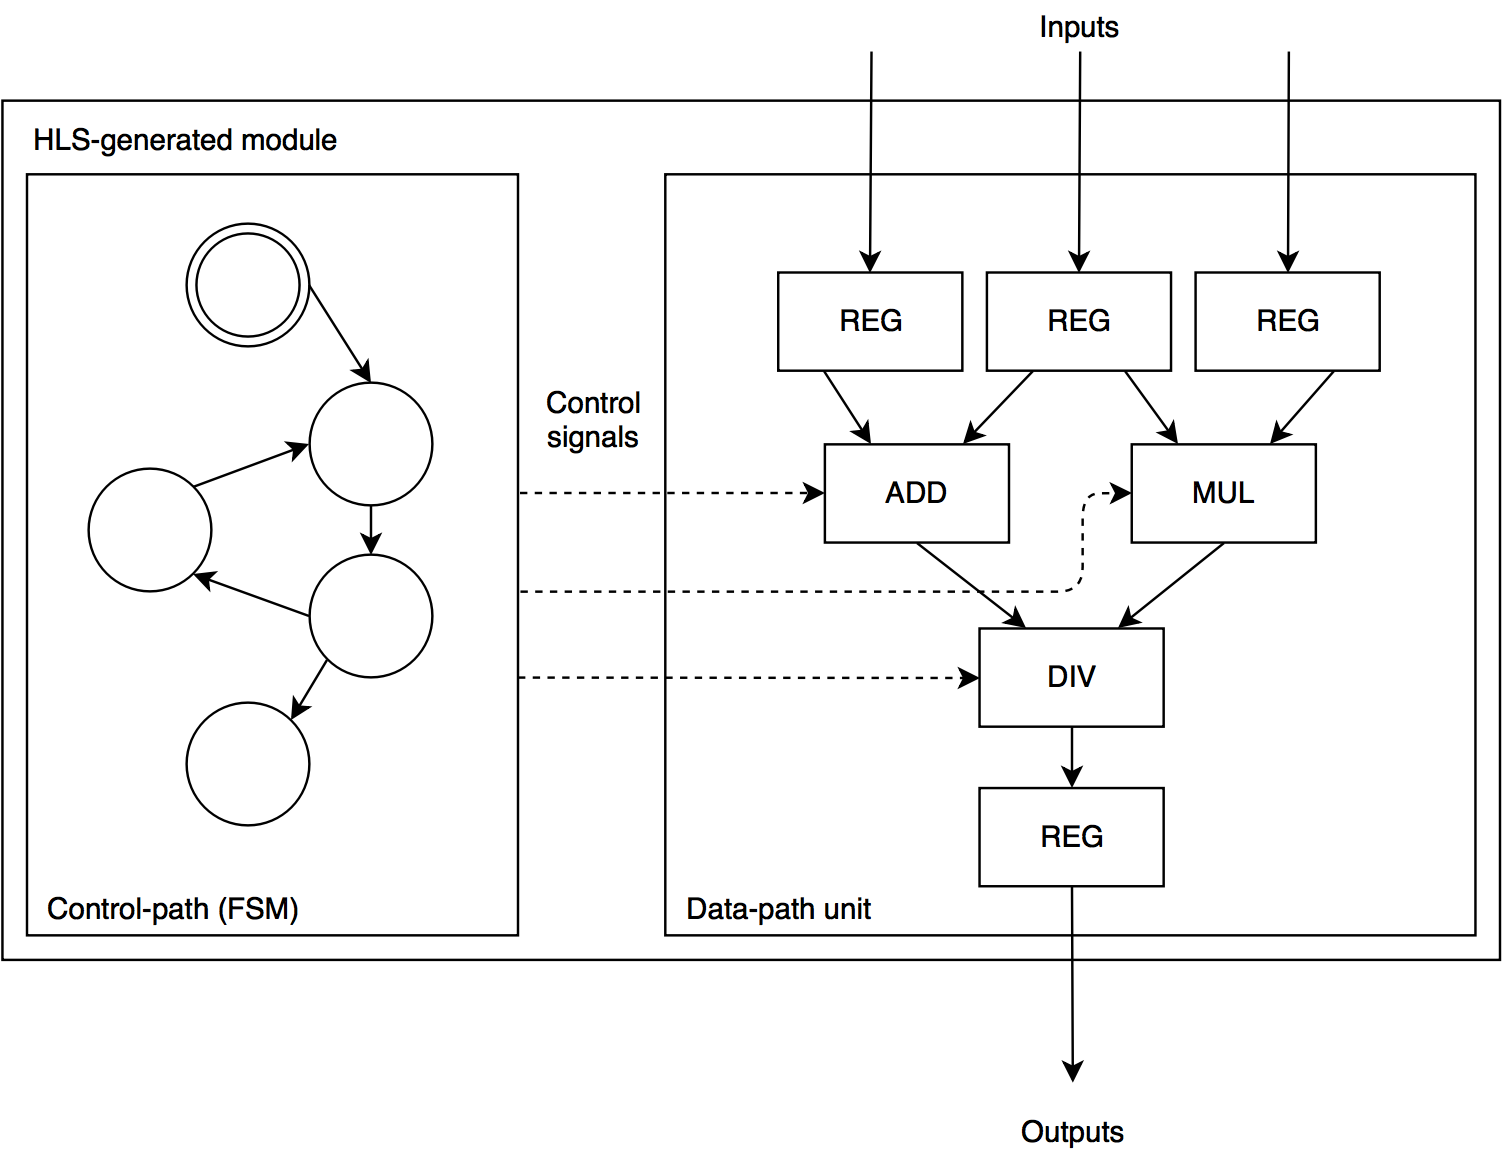
\includegraphics[width=0.65\textwidth]{../figs/HLSRTL.png}
\caption{\label{fig:hlsrtl}Typical division of control and data-path in the generated RTL from HLS.}
\end{figure}
Depending on the intensiveness of the binding step, the output \gls{rtl} can be tightly or loosely bound to the available resources. If an operation is not bound to a specific unit, it is up to the following logic synthesis of the \gls{rtl} to bind the operations to available resources. The different types of \gls{rtl} output are illustrated by the following example. \textit{a = b * c} executing in state \textit{n}:

\begin{minipage}[t][300px]{\textwidth}
\textbf{Without any binding:}%\hfill\vspace{-\baselineskip}
\begin{verbatim}
state (n): a = b * c;
go to state (n + 1);
\end{verbatim}
\textbf{With storage binding:}%\hfill\vspace{-\baselineskip}
\begin{verbatim}
state (n): S(1) = S(2) * S(3);
go to state (n + 1);
\end{verbatim}
\textbf{With functional-unit binding:}%\hfill\vspace{-\baselineskip}
\begin{verbatim}
state (n): a = MUL1 (b, c);
go to state (n + 1);
\end{verbatim}
\textbf{With storage and functional-unit binding:}%\hfill\vspace{-\baselineskip}
\begin{verbatim}
state (n): S(1)=MUL1 (S(2), S(3));
go to state (n + 1);
\end{verbatim}
\textbf{With storage, functional-unit, and connectivity binding:}%\hfill\vspace{-\baselineskip}
\begin{verbatim}
state (n): BUS1 = S(2); BUS2 = S(3);
BUS3 = MUL1 (BUS1, BUS2);
S(1) = BUS3;
go to state (n + 1);
\end{verbatim}
\end{minipage}

A loosely bound \gls{rtl} gives the synthesis-tool the flexibility to optimize the unit binding to updated timing estimates, delays, and loads given by the layout and floor-planning tools.

\section{LegUp}
The \gls{hls} tool used in this project is called LegUp \cite{canis2011legup}. LegUp is an open-source academic tool developed at the University of Toronto, Canada. LegUp's goal is to \textit{"allow researchers to experiment with new \gls{hls} algorithms without building a new infrastructure from scratch"} and their long-term vision is to \textit{"make \gls{fpga} programming easier for software developers"}. LegUp takes \gls{ansi}-C as input and generates synthesizable Verilog \gls{hdl} as output. The developers of LegUp have primarily focused on support for a variety of \gls{fpga} boards from manufacturer Altera, but in the latest version (4.0), beta support for Xilinx devices and possibility to configure the tool to generate generic Verilog to target other \gls{fpga} vendors or even \gls{asic} through use of generic dividers, has been introduced. The big advantage of LegUp compared to similar, commercial tools, is that it is open-source and therefore can be configured to target different architectures. The \gls{rtl} and \gls{hdl} generating part of the tool can be modified or replaced to fit the programmers needs.
Since LegUp, in its unmodified form, target \gls{fpga} devices, it support three different synthesis flows; pure-\gls{sw}, hybrid, and pure-\gls{hw}. The two first synthesis flows will implement a TigerMIPS \cite{tigmips} soft processor, which will run part of the C code. The partitioning of \gls{sw} and \gls{hw} in the individual modules are described in \cref{tab:legupflows}. It is the pure-\gls{hw} flow that will be the focus of this project.

\begin{table}[hbpt]
    \centering
    \caption{\label{tab:legupflows}HLS-flows supported by LegUp and partitioning between SW and HW}
    \begin{tabular}{lp{4.8cm}p{4.8cm}}
      \textbf{Flow} & \textbf{Functions run in hardware} & \textbf{Functions run in software}\\
      \toprule
      Pure-SW & None & All \\
      \hline
      Hybrid & Specified hardware-accelerated functions & All other functions \\
      \hline
      Pure-HW & All & None\\
      \bottomrule
    \end{tabular}
\end{table}

\subsection{Producing Verilog Output}
LegUp is made up of two components; a frontend pass and a target backend pass to the LLVM compiler infrastructure. 
The information flow in LegUp, shown in figure \ref{fig:legupflow}, follows the same principle as the information flow described in section \ref{sec:hls}.
\begin{figure}[hbpt]
\centering
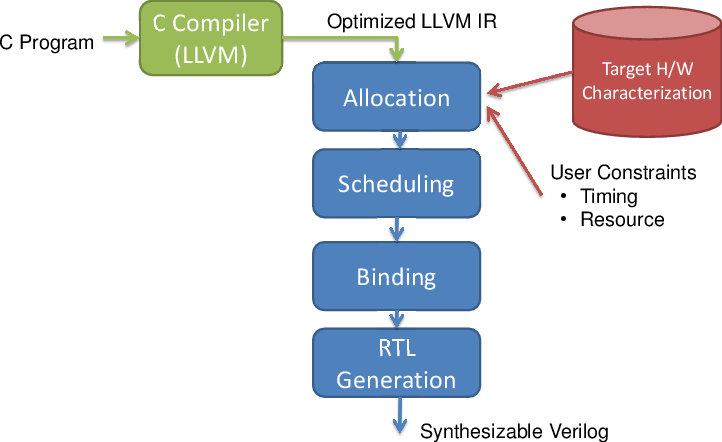
\includegraphics[width=0.6\textwidth]{../figs/LegUpFlow.png}
\caption{\label{fig:legupflow}Information flow in LegUp \cite{legupmaual}.}
\end{figure}
The LegUp LLVM frontend takes LLVM-\gls{ir} compiled by clang, a C frontend for LLVM, as input and links in custom written functions like memcpy, memset and memmove, which do not exist in hardware, but that LLVM assumes exist in the C library. 
The LegUp backend pass performs allocation, scheduling and binding as described in section \ref{sec:hls}. In the next step, \gls{rtl}-module objects that represents the final hardware circuit are generated from each LLVM instruction. Ultimately, Verilog code corresponding to each of the \gls{rtl}-modules is output to a file.

The allocation, scheduling, and binding in LegUp is performed based on information about available resources and timing information about the specified target FPGA-board, in addition to user-defined constraints and setting. The available information about the FPGA-boards allows for precise scheduling and binding to the available resources. Since the implementation of ASIC designs are quite different from the architecture and implementation of designs on FPGAs, the resource and timing information will not be as easily obtained for the target architecture. 

\subsection{\label{sec:legupclasses}Classes}
In LegUp there are some predefined classes that is important for the understanding of the description of adapting LegUp, described in \cref{chp:adaptinglegup}. The following subsections will describe some important information about these classes in more detail. The full class descriptions can be found in the \textit{LegUp Namespace Reference} \cite{legupclassref}.
\subsubsection{RTLModule}
The RTLModule class models a hardware RTL module. The class stores information about all ports (inputs and outputs), signals, parameters and sub-modules. Each function declared in the C-code transforms into a RTLModule object. Each function that is called from the function will be added as a sub-module to the RTLModule object, meaning a module instantiation will be added to the module. Important member-functions of the RTLModule class are:
\begin{compactdesc}
    \item[getName()] \hfill \\
    Returns a string containing the name of the RTLModule, i.e. "main" for the module generated by the \textit{main}-function in the C-program.
    \item[find(std::string signal)] \hfill \\
    Takes a string containing a signal name as parameter and returns a pointer to the RTLSignal in the RTLModule with that name.
    \item[addParam(std::string name, std::string value)] \hfill \\
    Adds a parameter to the module. The function returns a pointer to the generated RTLSignal object.
    \item[addIn(std::string name, RTLWidth width)] \hfill \\
    Adds an input-port to the module. The function returns a pointer to the generated RTLSignal object.
    \item[addOut(std::string name, RTLWidth width)] \hfill \\
    Adds an output-port to the module. The function returns a pointer to the generated RTLSignal object.
    \item[addRegOut(std::string name, RTLWidth width)] \hfill \\
    Adds a registered output port to the module. The function returns a pointer to the generated RTLSignal object.
    \item[addReg(std::string name, RTLWidth width)] \hfill \\
    Adds a register signal to the module. The function returns a pointer to the generated RTLSignal object.
    \item[addWire(std::string name, RTLWidth width)] \hfill \\
    Adds a wire signal to the module. The function returns a pointer to the generated RTLSignal object.
    \item[addModule(std::string name, std::string instName)] \hfill \\
    Adds an instantiation of another module to the module. The function returns a pointer to the generated RTLModule
    object.
\end{compactdesc}
\subsubsection{RTLSignal}
The RTLSignal class represents the signals within an RTLModule. Both internal signals, port signals and condition signals are all modelled using the RTLSignal class. Important member-functions of the class are:
\begin{compactdesc}
    \item[getName()] \hfill \\
    Returns a string containing the name of the RTLSignal, i.e. "clk" for the clock signal.
    \item[getType()] \hfill \\
    Returns a string describing the signal type. The type can be \textit{reg}, \textit{wire}, \textit{input}, \textit{output}, or \textit{output reg}.
    \item[getNumDrivers()] \hfill \\
    Return the number of driving RTLSignals. 
    \item[getDriver(unsigned i)] \hfill \\
    Returns a pointer to the i-th driving RTLSignal.
    \item[getCondition(unsigned i)] \hfill \\
    Returns a pointer to the condition signal of the i-th driving RTLSignal.
    \item[addCondition(RTLSignal *cond, RTLSignal *driver)] \hfill \\
    Adds a conditional driver. If the RTLSignal \textit{cond} is true, the RTLSignal \textit{driver} drives the signal. 
    \item[connect(RTLSignal *s)] \hfill \\
    Connect this signal unconditionally to another RTLSignal.
    \item[getWidth()] \hfill \\
    Returns a pointer to a RTLWidth object, describing the width of the RTLSignal.
    \item[isOp()] \hfill \\
    Returns true if the RTLSignal is an RTLOp object.
\end{compactdesc}
\subsubsection{RTLOp}
The RTLOp class is a subclass of the RTLSignal class, representing an operation with one, two or three operands. Each operand is a RTLSignal. The operation can be an arithmetic operation like addition, subtraction, multiplication, or division, and it can also be logical operations like AND, OR, and XOR, or even comparison operations like equal, not equal, less than, less than or equal, greater than, and greater than or equal. The whole list can be seen in the class reference \cite{rtlopclassref}. A RTLOp object modelleing an AND operation of two operands, operand1 and operand2, will in Verilog correspond to the operation "\verb!operand1 & operand2!". Some important member-functions are:
\begin{compactdesc}
    \item[getOperand(int i)] \hfill \\
    Returns a pointer to i-th operand of the RTLOp object.
    \item[getNumOperands()] \hfill \\
    Returns the number of operands of the RTLOp object.
    \item[setOperand(int i, RTLSignal *s)] \hfill \\
    Sets the i-th operand to the RTLSignal \textit{s}.
\end{compactdesc}
\subsubsection{RTLWidth}
The RTLWidth class represents the bitwidth of a RTLSignal. An RTLWidth is defined by high and low bits, for instance 31,0 for a 32 bit signal. This will transform into "\verb![31:0]!" in Verilog.
\subsubsection{RAM}
The RAM class models RAM modules in LegUp. Whenever a variable is loaded or stored, a RAM module is generated to handle the loads and stores. The RAM objects can be divided into two scopes; LOCAL and GLOBAL. A Local RAM object is local to a given function and cannot be accessed from other functions. A global RAM object will be implemented in a global memory controller. All modules that use the variable can connect to the RAM via the memory controller. Some important member-functions are:
\begin{compactdesc}
    \item[getName()] \hfill \\
    Returns a string containing the name of the RAM module, i.e. "main\_0\_1" for the RAM module generated for the first parameter to the main function declared as volatile (output parameters) in the C-code.
    \item[isROM()] \hfill \\
    Returns true if the RAM is read-only.
    \item[getScope()] \hfill \\
    Returns if the RAM is in the local or global scope.
\end{compactdesc}


\subsection{\label{subsec:legupconstraintstheory}Constraints}
Constraints is an important part of LegUp, and it is also used extensively in this project. The constraints are used for setting design goals and limitations on design, and to specify how the \gls{hls}-flow shall be executed. Constraints play an important role in this concept, as the idea is to generate multiple designs that can be compared in terms of area, speed, and power consumption. For the designs to be different, varying constraints are used for generating the designs. All available constraints are described in the constraint manual \cite{legupconst}, but the ones used in this project are described in \cref{tab:constraintssescription}. Some constraints are considered \textit{required}. These constraints must be set for the generated design to be compatible with the tool-flow. \textit{HLS constraints} are used for getting different Verilog output from LegUp. Other constraints from the constraint manual can be also be used, but these were selected for this project as their description indicate that they can affect the architecture of the output.
\begin{table}[hbtp]
    \centering
    \begin{tabular}{l|p{6.4cm}|c}
    \multicolumn{3}{c}{\textbf{Required constraints}} \\
    \toprule
    \multicolumn{1}{c}{\textbf{Parameter name}} & \multicolumn{1}{c}{\textbf{Description}} & \specialcell{\textbf{Required}\\\textbf{value}} \\
    \midrule
    \small{DIVIDER\_MODULE} & Use generic divider module rather than Altera primitive & \textit{generic} \\
    \hline
    \specialcelll{\small{EXPLICIT\_}\\\small{LPM\_MULTS}} & Use Altera primitive multiplier rather than Verilog multiply operator (*) & \textit{0} \\
    \hline
    \small{INFERRED\_RAMS} & Use Verilog inferred RAMs rather than Altera altsyncram modules & \textit{1} \\
    \hline
    \specialcelll[t]{\small{INFERRED\_}\\\small{RAM\_FORMAT}} & Select format of inferred RAMs. Altera: multiple always blocks, Xilinx: same always block & \textit{xilinx} \\
    \hline
    \small{LOCAL\_RAMS} & Infer all RAMs as local RAMs rather than global RAMs. RAMs being accessed by multiple functions will override this setting & \textit{1} \\
    \hline
    \small{VSIM\_NO\_ASSERT} & Disable triple-equality assertions. This causes simulation to fail & \textit{1} \\
    \midrule
    \multicolumn{3}{c}{\textbf{HLS constraints}} \\
    \toprule
    \multicolumn{1}{c}{\textbf{Parameter name}} & \multicolumn{2}{c}{\textbf{Description}} \\
    \midrule
    \small{SDC\_NO\_CHAINING} & \multicolumn{2}{p{8cm}}{Schedule each operations into a separate clock cycle} \\
    \hline
    \small{MB\_MINIMIZE\_HW} & \multicolumn{2}{p{8cm}}{Run LegUp-pass that tries to minimize signal sizes} \\
    \hline
    \small{CASE\_FSM} & \multicolumn{2}{p{8cm}}{Use case-statements in FSM rather than If-Else} \\
    \hline
    \small{PIPELINE\_ALL} & \multicolumn{2}{p{8cm}}{Enable pipelining for all loops, regardless of loop-label} \\
    \hline
    \specialcelll{\small{ENABLE\_}\\\small{PATTERN\_SHARING}} & \multicolumn{2}{p{8cm}}{Turn on resource sharing for patterns in \gls{dfg}} \\
    \hline
    \specialcelll{\small{DUAL\_PORT\_}\\\small{BINDING}} & \multicolumn{2}{p{8cm}}{Use dual-ported on-chip memories} \\
    \bottomrule
    \end{tabular}
    \caption{Descriptions of constraints used in this project}
    \label{tab:constraintssescription}
\end{table}

\section{\label{sec:LLVM}LLVM}
LLVM \cite{LLVM:CGO04}, formerly Low-Level Virtual Machine, is a compiler framework that was originally developed as a research infrastructure to investigate dynamic compilation techniques for static and dynamic programming languages, at the University of Illinois in 2000. It is now a open-source project with many contributors from both industry, research groups and individuals, and it is used by companies like Apple in their Xcode \gls{ide} \cite{llvmapple} and Sony for their PS4 developer toolchain \cite{llvmsony}. LLVM support a large number of frontends for programming languages, including Clang \cite{clang} which support C, C++, Obcjective-C, and Objective-C++, and is compatible with \gls{gcc}. It also supports a large number of backend target architectures. Figure \ref{fig:llvmcompiler} shows how different source languages can be input to the frontend compilers of LLVM, which translate the source into an \gls{ir}. The \gls{ir} is then optimized using LLVM's optimizer. At this stage, different source languages can be linked together, and even object files compiled using standard \gls{gcc} can be linked at this stage. The optimized \gls{ir} is then translated into the target architecture by the backend.

\begin{figure}[hbpt]
\centering
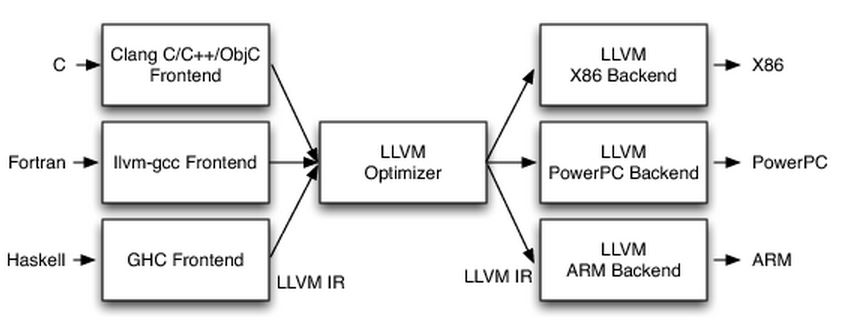
\includegraphics[width=\textwidth]{../figs/LLVMCompiler.jpg}
\caption{\label{fig:llvmcompiler}LLVM's three-phase compiler structure \cite{llvmarch}.}
\end{figure}

\subsection{Intermediate Representation}
LLVM use a human readable, assembly-like, strongly typed RISC instruction set as their \gls{ir}, with support for an infinite number of temporary registers of the form \%0, \%1, etc. LLVM-\gls{ir} can also output a dense bitcode format for serialization. Conversion between the bitcode-format and the human-readable format, and vice versa, can be done with the commands "\verb!llvm-dis!" and "\verb!llvm-as!", for dis-assembly and assembly.

Some parts of the LLVM \gls{ir} will be described in \cref{chp:toolflowex}. The whole language are too large to be fully explained here, but interested readers can read more about the syntax in the \textit{LLVM Language Reference Manual} \cite{llvmlangman}.

\section{Alternative hardware design methods}
\gls{hls} is not the only alternative to \gls{hdl}-languages, if you want to design digital hardware at a higher level of abstraction. The following subsections will shortly describe two alternative approaches to digital hardware design. 
\subsection{Chisel}
One interesting approach to designing hardware with a higher level of abstraction, is the Chisel \gls{hcl} \cite{bachrach2012chisel}, developed at UC Berkeley. \gls{hdl} languages like VHDL and Verilog, were originally designed as simulation languages and later adopted as a basic for synthesis. Chisel, on the other hand, was created as a \gls{hcl} and is thus \textit{synthesizable by construction}. This entails that no conversion from C, or other \gls{hll}, into gates is performed, only generation of generic low-level Verilog with no overhead. Chisel is a \gls{dsl} built on Scala \cite{odersky2004overview} with its own syntax, but Scala syntax can also be used to get even greater abstraction in your design. A big advantage using Chisel is its high simulation speed, using C++-based cycle-accurate software simulators.

\subsection{Functional programming}
Functional programming is a relatively different method of hardware design, as it consists only of mathematical functions and immutable data. Two examples of hardware design using functional programming is C$\lambda$aSH \cite{baaij2009clash} and Lava \cite{bjesse1998lava}. Both Lava and C$\lambda$ash are compilers for the functional programming language Haskell \cite{haskellonline}, but while Lava is an embedded \gls{dsl} like Chisel, with its own syntax, C$\lambda$ash use Haskell syntax and semantics, and use a static analysis approach towards synthesis.

\section{\label{sec:powdiss}Power dissipation in CMOS circuits}
The power dissipation in CMOS circuits can be divided into three categories \cite{panda2010power}, \textit{dynamic power}, \textit{short-circuit power} and \textit{leakage power}. This gives a total power dissipation of:
\begin{equation}
    P_{total} = P_{dynamic} + P_{short-circuit} + P_{leakage}
\end{equation}

Figure \cref{fig:powerdisscmos} shows the distribution of the power components of the CMOS circuit. Each component is described in more detail in the following subsections, where \textit{switching power} corresponds to $P_{dynamic}$, \textit{internal power} corresponds to $P_{short-curcuit}$, and \textit{leakage power} to $P_{leakage}$.
\begin{figure}[hbpt]
\centering
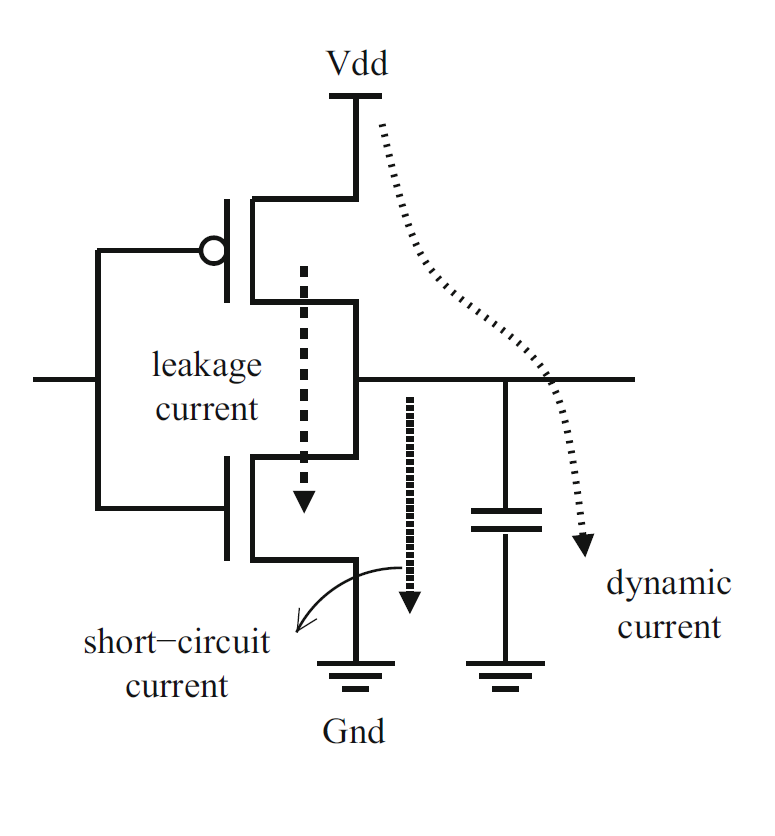
\includegraphics[width=0.4\textwidth]{../figs/PowerDissipation.png}
\caption{\label{fig:powerdisscmos}Power dissipation components distribution \cite{panda2010power}.}
\end{figure}

\subsection{Switching power}
Whenever a signal change the logic state from 0 to 1, causing the load capacitance to be charged by the power supply. The power dissipated during this process is called \textit{Switching power}. Half the energy drawn from the power supply needed to charge the capacitance, is dissipated as heat in the process. The \textit{switching power} depends on the frequency of the switching, the switching factor of gates, and the load capacitance, in addition to the supply voltage. 

\subsection{Internal power}
The \textit{internal power} is the power used to charge and discharge the internal capacitance of the circuits, whenever a pin changes its logic state. A large part of the \textit{internal power} is the short-circuit power. In the short time when both the pMOS and nMOS transistor of the CMOS circuit is \textit{on}, a current will be drawn from the source $V_{dd}$ to $Gnd$, through the short-circuit that will occur. 

\subsection{Leakage power}
Whenever the circuits are turned \textit{on}, a small leakage current will be drawn from the gates. The leakage power is mostly caused by sub-threshold currents and reverse biased diodes in the circuits. The leakage current increase when the technology shrinks, making leakage a bigger problem today than before. 

\section{\label{sec:toolflowbg}Tool-flow}
This section will describe all the tools that are used throughout this thesis, as well as the connection and data-flow between the different tools. This flow is based on the standard tool-flow used at Nordic Semiconductor, and it include some parts adapted from the "\textit{automated area and power estimation tool-flow}" created by Joar Talstad for his Master thesis \cite{talstad15master}. Most of the tool-flow is based on scripts and Makefiles that can be run from a Linux shell, but there are also some GUI-tools available that will be mentioned briefly in \cref{chp:toolflowex}. The following subsection will describe the different sections of the tool-flow in detail. The flow in LegUp will not be described here, as this is covered above and will be presented in more detail in \cref{chp:toolflowex}.

\subsection{Simulation}
Simulation is run to verify the correctness of a design and to help detect and eliminate potential bugs. In this project, the simulation tool also generates a \gls{vcd}-file, \textit{designname.vcd}, showing switching activity during simulation. This file is used in the power analysis tool later in the flow, to get a realistic input of the amount of switching in the design. Simulation is performed using the tool ModelSim for Questa-64, version 10.2b 2013.05 \cite{questasim}. Simulation is executed by calling the script \textit{RUN\_ALL}. The \gls{rtl}-design filelist and a file containing a testbench module must be specified in the filelist found in the \textit{sim/tb/}-directory. This is used as input to the simulation tool.
\subsection{Synthesis}
Synthesis translates a \gls{rtl}-design written in a \gls{hdl}-language, like Verilog or VHDL, into a netlist for a specified target library. The tool used for synthesis in this thesis is Synopsys Design Compiler, version I-2013.12-SP2 \cite{syndescomp}. A cell library describing 180nm technology is used as the target architecture. A Makefile is used to start synthesis, and the command \verb!make compile! runs the full synthesis. The netlist generated by synthesis is found in the file \textit{designName.mapped.v} in the \textit{result}-directory. This netlist is used as input for the layout-tool. Synthesis generate reports showing area-estimates, register count, critical path and static power estimates for the design. As the design will be processed further through the tool-flow, these reports are not that accurate and hence not that useful.
\subsection{Layout}
Layout translates the netlist generated during synthesis into a chip layout. The tool used for layout in this project is Synopsys IC Compiler, version L-2016.03-SP1 \cite{syniccomp}. A Makefile is used to start layout, and the command \verb!make outputs_cts! runs the correct layout-script. Layout produces a new netlist-file, stored in the file \textit{designName.output.v} in the \textit{result}-directory. This netlist is used in the power analysis tool for estimating power consumption. Layout generate reports about area and critical paths, stored in the \textit{reports}-directory. These results are more accurate, as they were gathered from the actual chip layout.
\subsection{\label{sec:powest}Power analysis}
Power analysis is performed to get an early indication on how much power the final chip will be consuming. The tool used for power analysis in this thesis is Synopsys Primetime, version K-2015.12-SP3. To get accurate power estimates, the switching activity file generated during simulating is used together with the netlist output from layout. The conclusion from \cite{talstad15master} were that this method is well suited for making RTL-design trade-offs based on power consumption in multi-voltage designs, and provides accurate results. Power analysis is run on five different power scenarios, each giving a separate result for each of the three power dissipation categories described in \cref{sec:powdiss}. The reports are stored in the \textit{reports}-directory.

\section{Reference design}
\label{sec:refdes}
This thesis will look into whether or not LegUp can be used as the HLS-tool in a framework for architectural exploration of hardware. In order to get some output from LegUp than can be compared towards each other, a reference design must be created. The design will be used in the proof-of-concept, described in \cref{chp:frameworkresults}, and should be something that can be implemented both in C and Verilog. The design should also be simple to implement and verify. In \cite{holm2015pro}, two reference designs were implemented; a FIR-filter and a SAP-1 architecture. The FIR-filter will be used as the reference design in this project, as this is a regular structure that easily can be implemented and verified. The SAP-1 architecture would have been a interesting second reference design, as it consists of a FSM, just like the output from LegUp. Unfortunately, this architecture has too many design-parts that will be incompatible with the framework.

\subsection{\label{subsec:refdesfir}FIR-filter}
\gls{fir}-filters are together with \gls{iir}-filters, the two categories of linear time-invariant systems, used in digital signal processing application. The impulse response of a \gls{fir}-filter is zero outside some finite time interval. 
A general \gls{fir}-filter can be described by the differential equation \cite{proakis2007digital}:
\begin{equation}
    y(n)=\sum\limits_{k=0}^{M-1} b_kx(n-k)
    \label{eq:firfilterdiff}
\end{equation}
or by the system function:
\begin{equation}
    H(z)=\sum\limits_{n=0}^{M-1} b_nz^{-n}
    \label{eq:firfiltersys}
\end{equation}
The impulse response for a \gls{fir}-filter is given by:
\begin{equation}
    h(n)\triangleq
    \begin{cases}
    \begin{tabular}{ll}
      $0,$ & $n < 0$  \\
      $b_n,$ & $0 \leq n \leq M-1$  \\
      $0,$ & $n > M$   
      \end{tabular}
    \end{cases}
    \label{eq:firfilterimp}
\end{equation}
From \cref{eq:firfilterdiff} and \cref{eq:firfilterimp} we get the discrete convolution equation:
\begin{equation}
    y(n)=\sum\limits_{k=-\infty}^{\infty} h(k)x(n-k) \triangleq h(n) \ast x(n)
    \label{eq:firfilterconv}
\end{equation}
\noindent
Figure \ref{fig:firfilter} shows the direct form representation of a N-order \gls{fir}-filter with $N+1$ taps. The figure shows that a FIR-filter requires $N$ memory elements, $N+1$ adders and \textit{N} multipliers. 
\begin{figure}[hbpt]
\centering
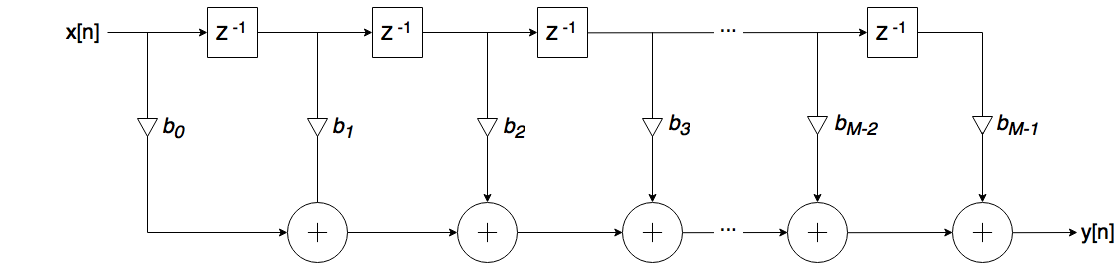
\includegraphics[width=\textwidth]{../figs/FIRFilter.png}
\caption{\label{fig:firfilter}Direct form representation of a N-order FIR-filter.}
\end{figure}


Even though the process of designing a \gls{fir}-filter might not be a trivial task, the implementation of an already designed filter is simple. As seen from \cref{eq:firfilterconv}, the filter can be described by the convolution formula, which implies that the filter can be implemented as convolution of the input function \textit{x(n)} with the impulse response function \textit{h(n)}.